\documentclass[UTF8]{ctexbeamer}

\usepackage[backend=bibtex,sorting=none]{biblatex}
\addbibresource{reference.bib}
\setbeamerfont{footnote}{size=\tiny}

\usetheme{Warsaw}
\useoutertheme{miniframes}

\title{AI for System and System for AI}
\author{Conless Pan}
\date{\today}

\begin{document}

\begin{frame}[plain]
  \titlepage
\end{frame}

\begin{frame}
  \tableofcontents
\end{frame}

\section{Introduction}

\begin{frame}{The Rise of Machine Learning}
  \begin{center} 
    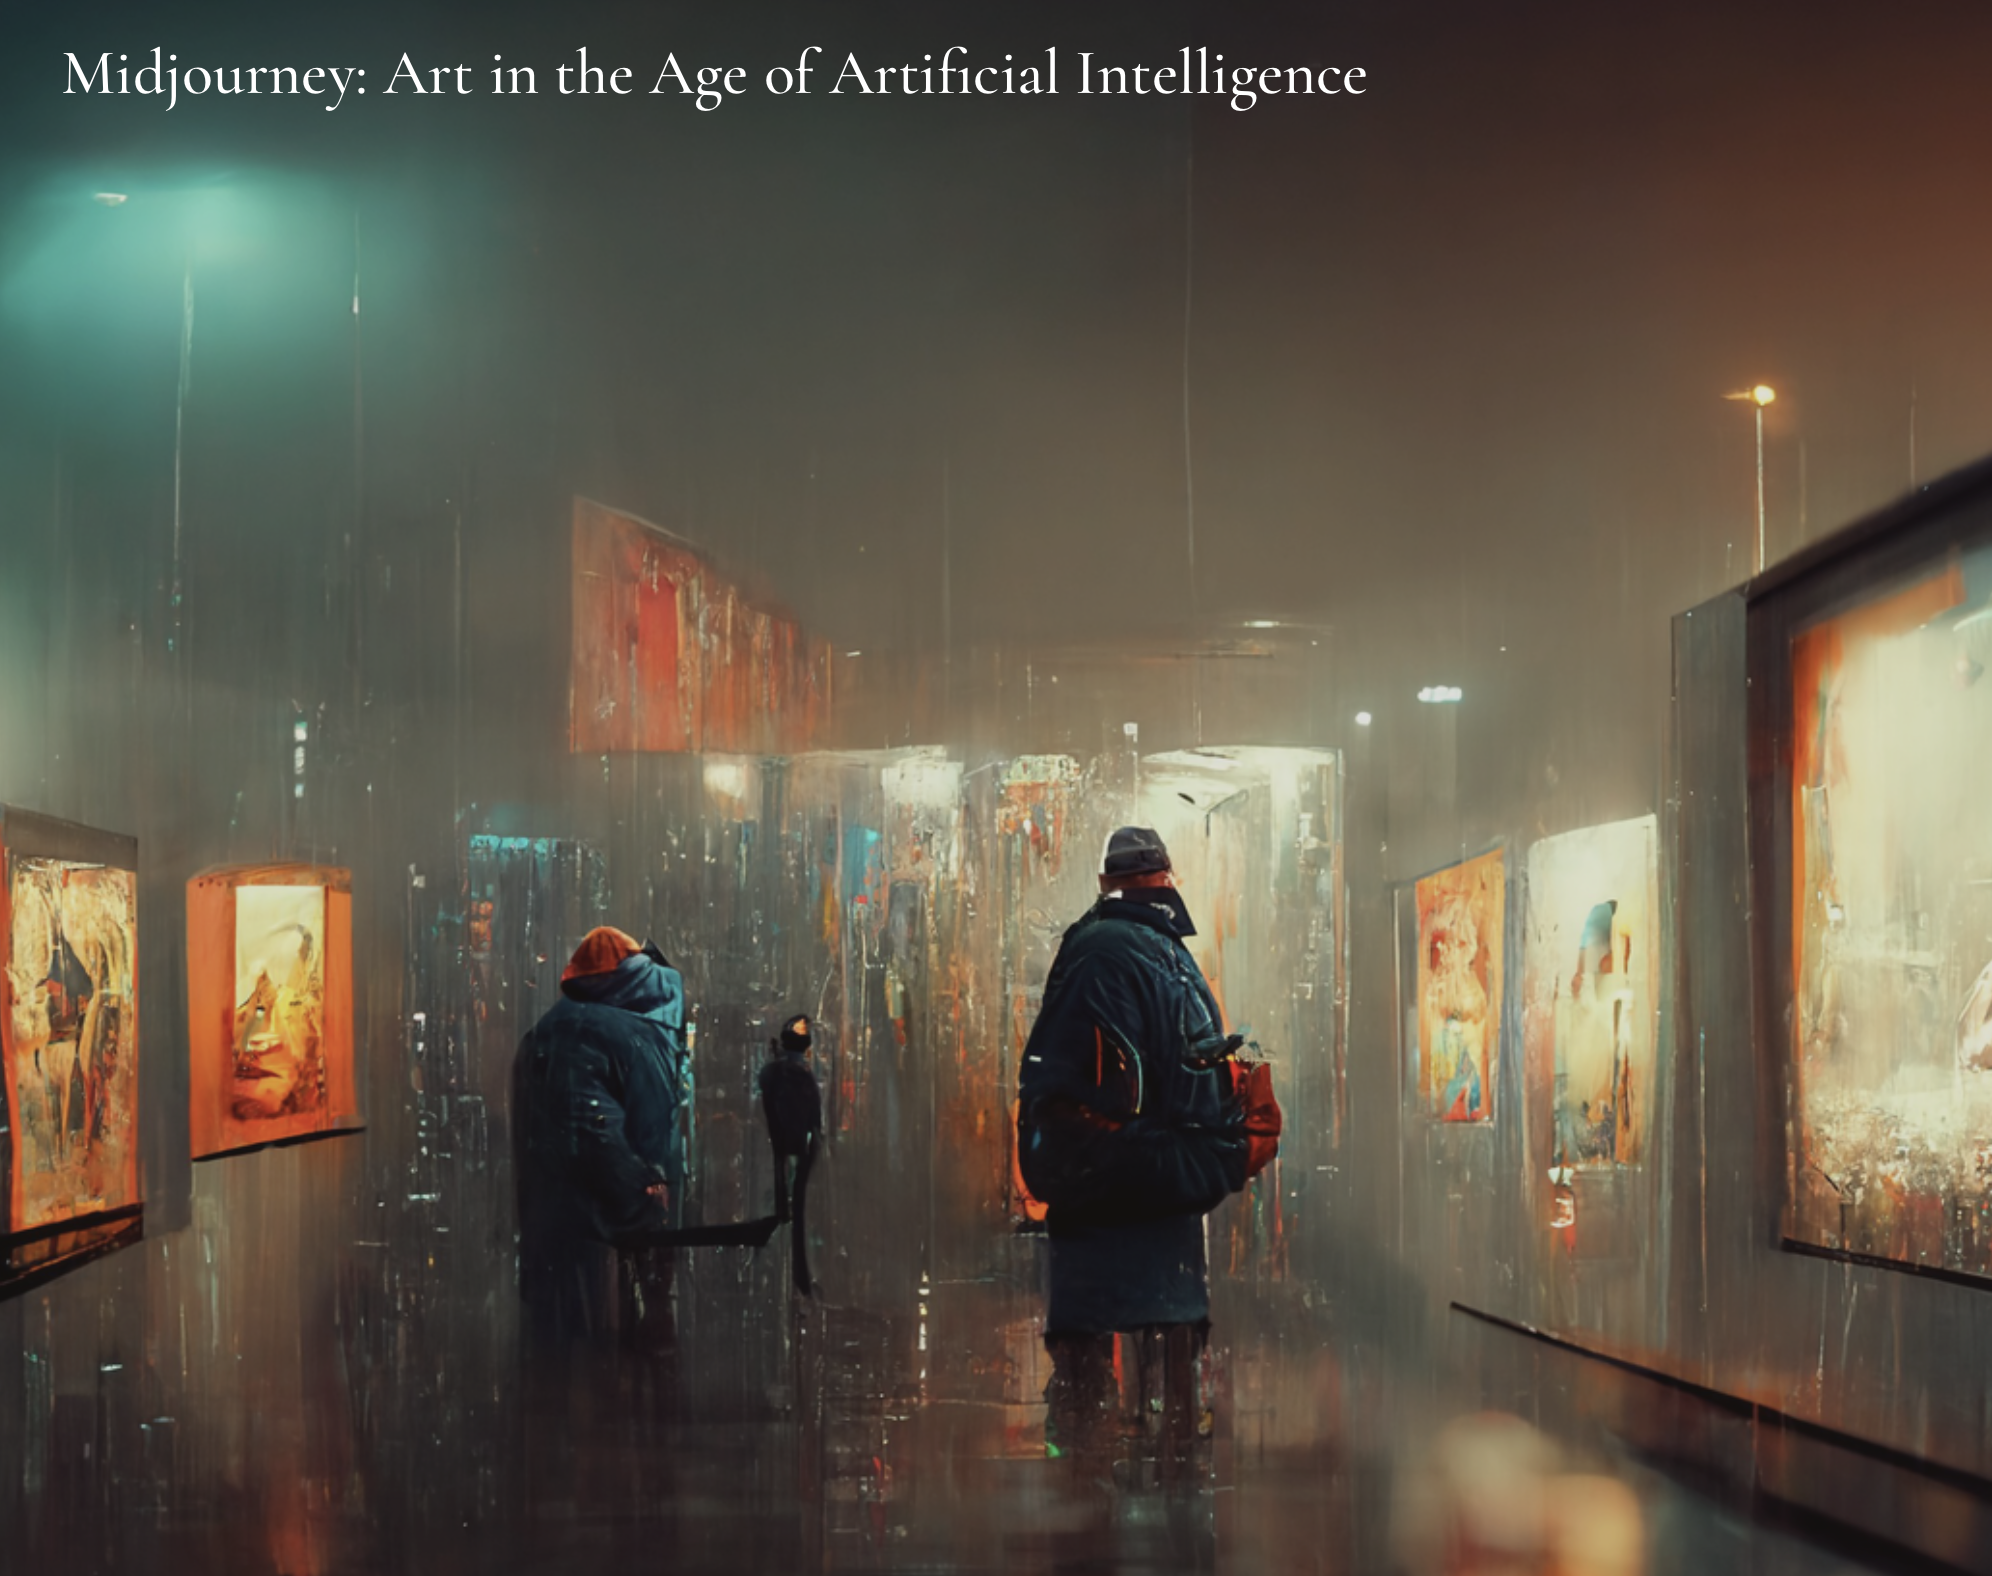
\includegraphics[height=150pt]{figure/midjourney_home.png} 
    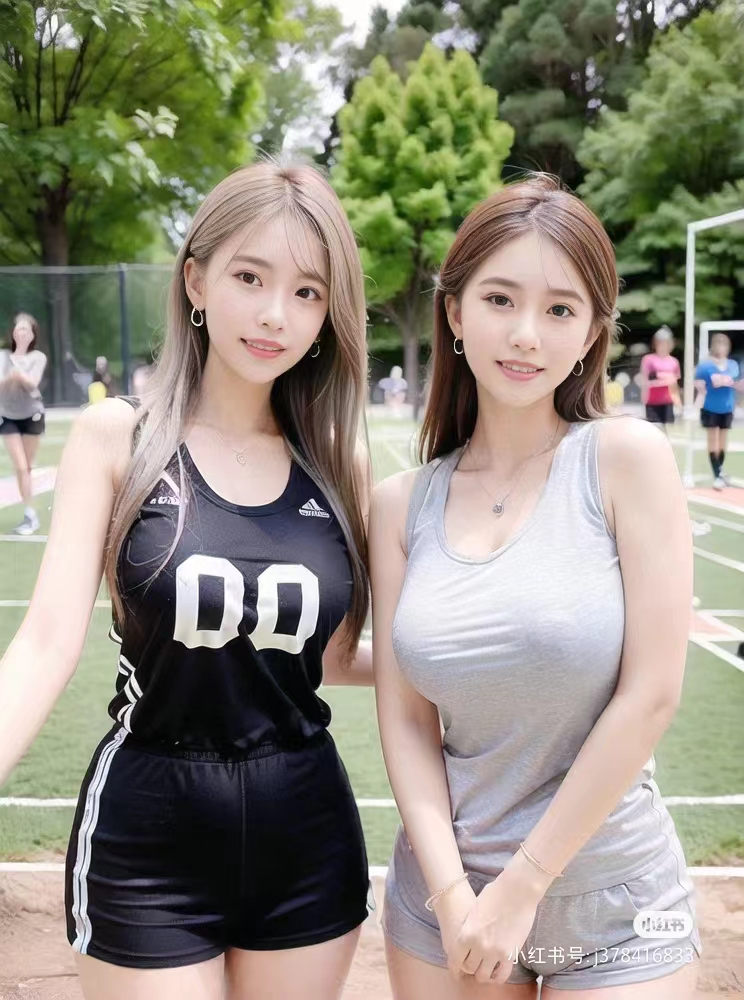
\includegraphics[height=150pt]{figure/ai_pic.jpg} 
  \end{center}  
\end{frame}

\begin{frame}{The Rise of Machine Learning}
  \begin{center}
    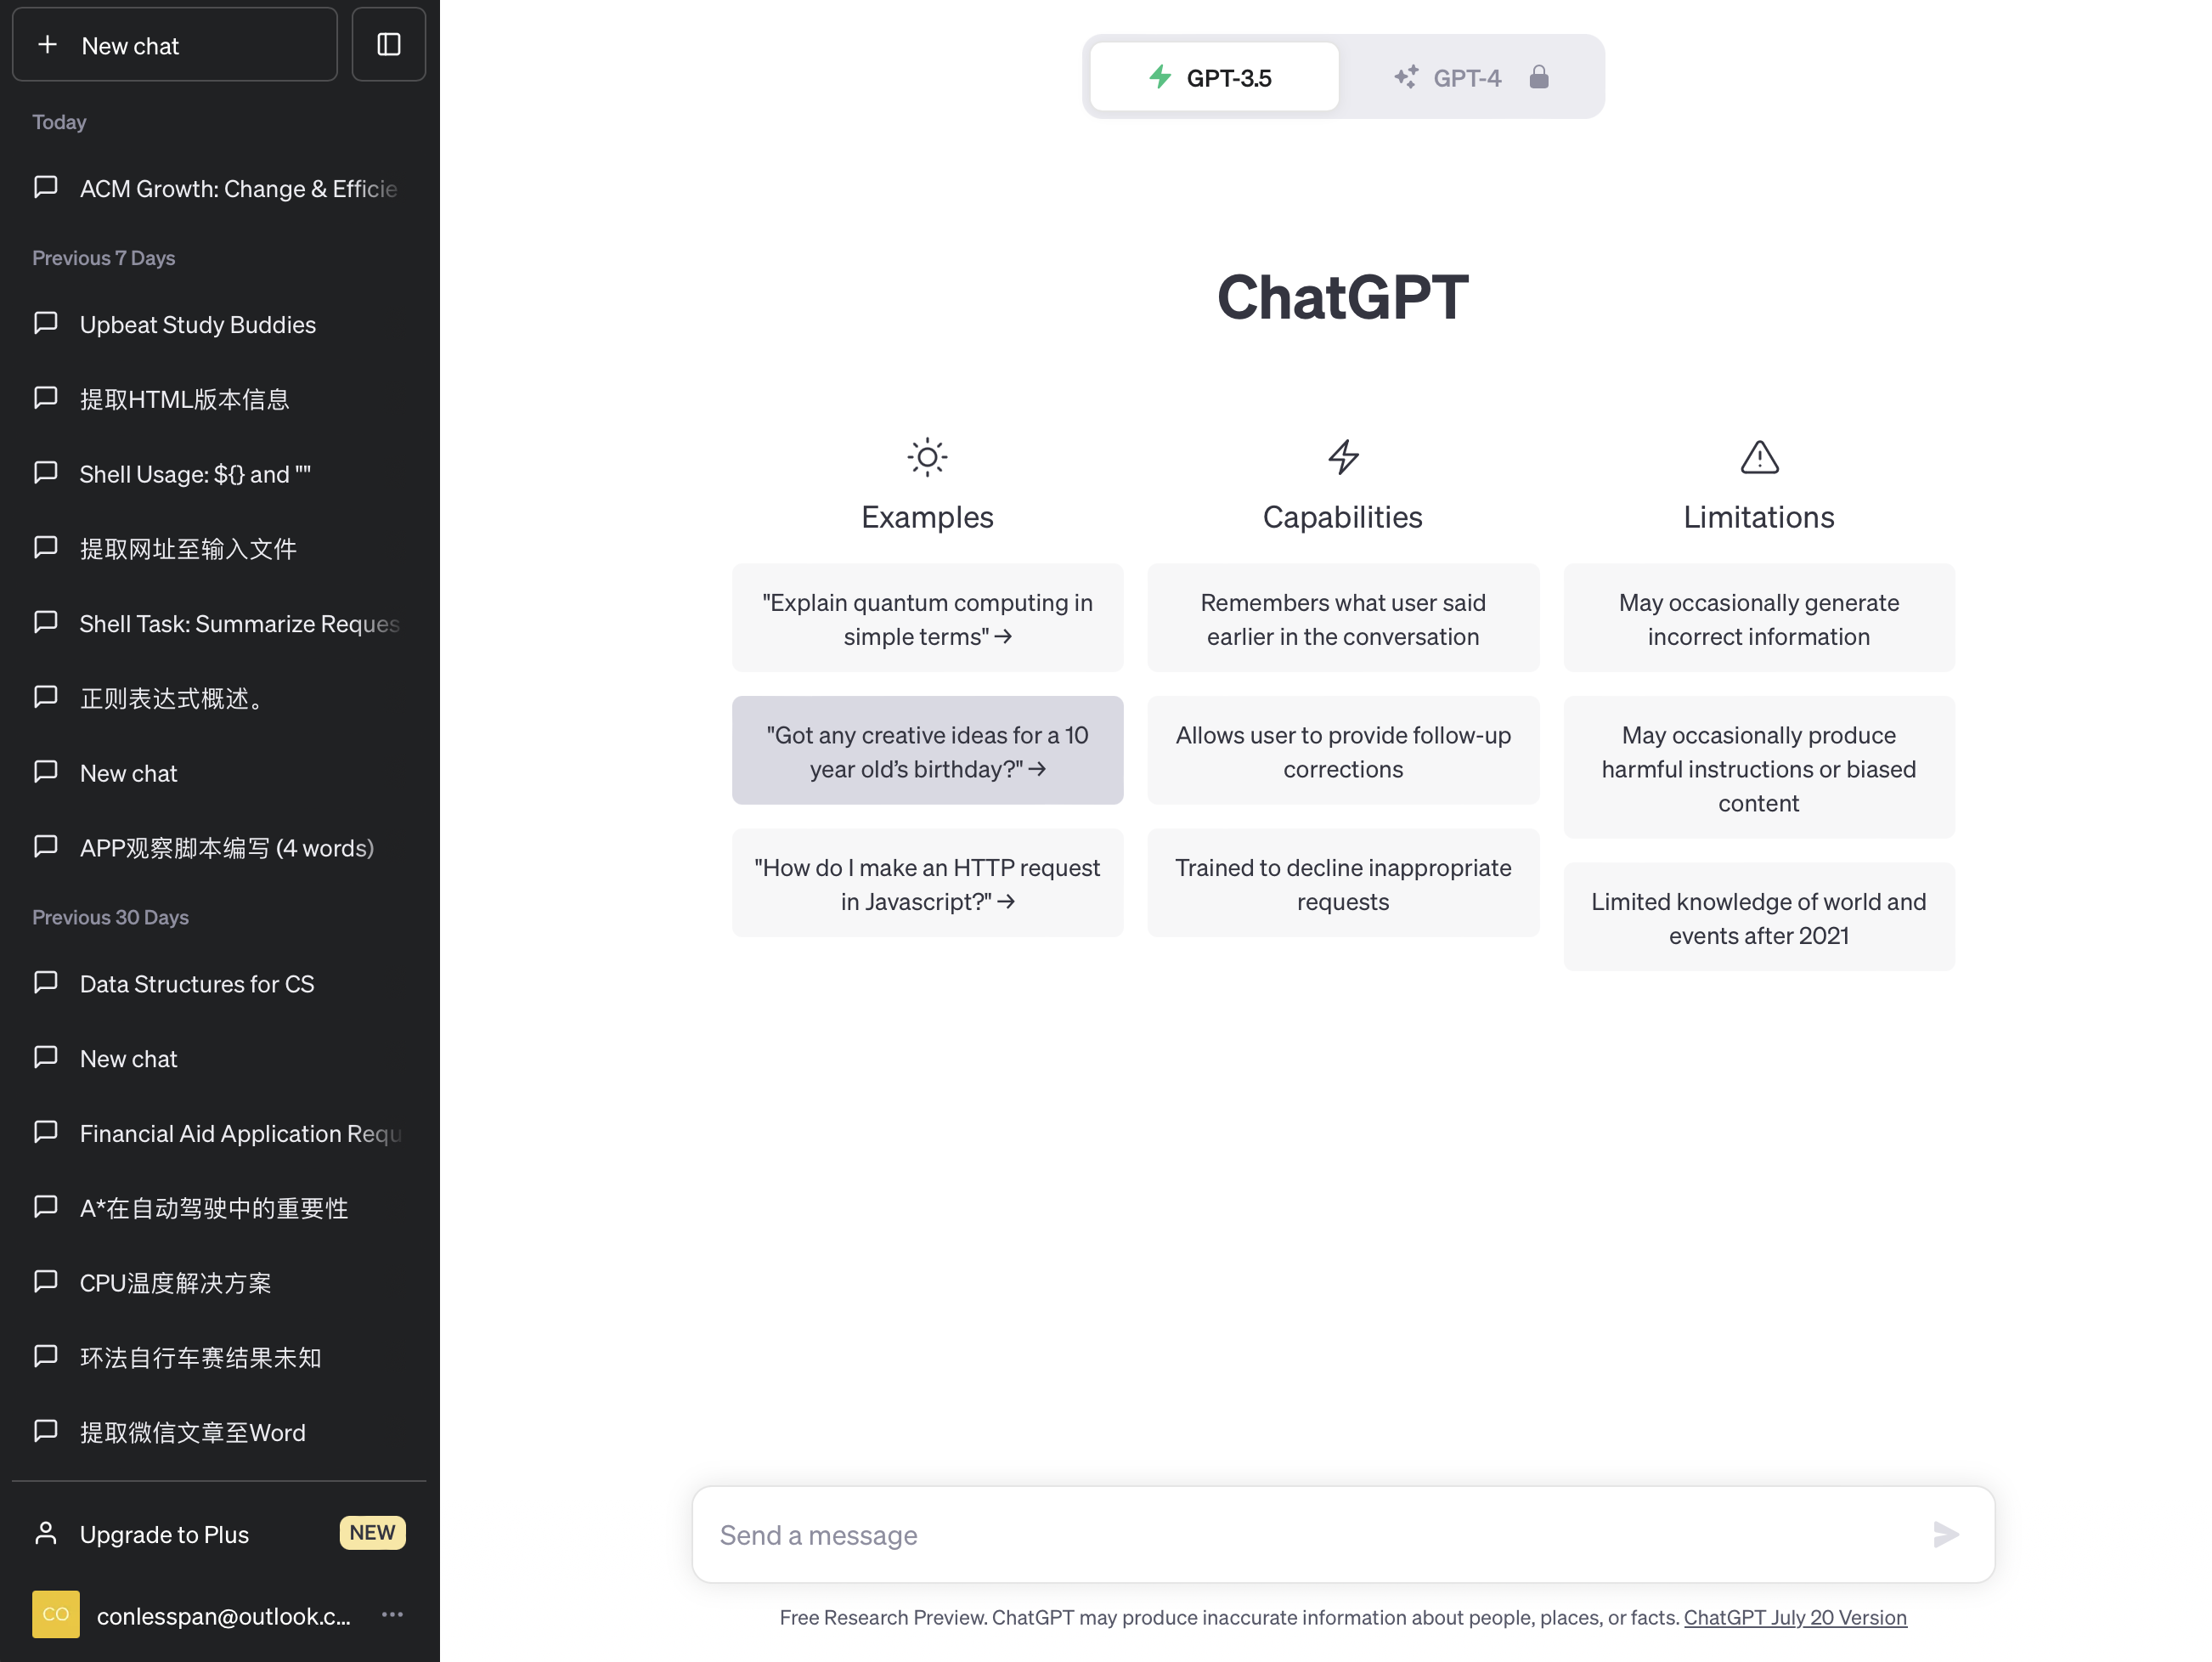
\includegraphics[height=200pt]{figure/chatgpt.png}
  \end{center}
\end{frame}

\begin{frame}{The Rise of Machine Learning}
  \onslide<1->{When we talk about the rise of machine learning, people usually raise these questions:}
  \begin{itemize}
    \item<2-> What is machine learning?
    \item<3-> Do you know its history?
    \item<4-> Why is it so important today?
  \end{itemize}
  \onslide<5->{But I don't want to talk about them, cause I'm not interested about AI.}
\end{frame}

\begin{frame}{Applications of Machine Learning}
  Anyway, AI is a useful tool.
  \begin{itemize}
    \item<2-> Generative AI
    \item<3-> AI for science
    \item<4-> Others
  \end{itemize}
\end{frame}

\section{AI for System}

\begin{frame}{How can AI promote our research of computer system?}
  Let's compare these two games:\footfullcite{smith1998study}
  \begin{center} 
    \onslide<2->{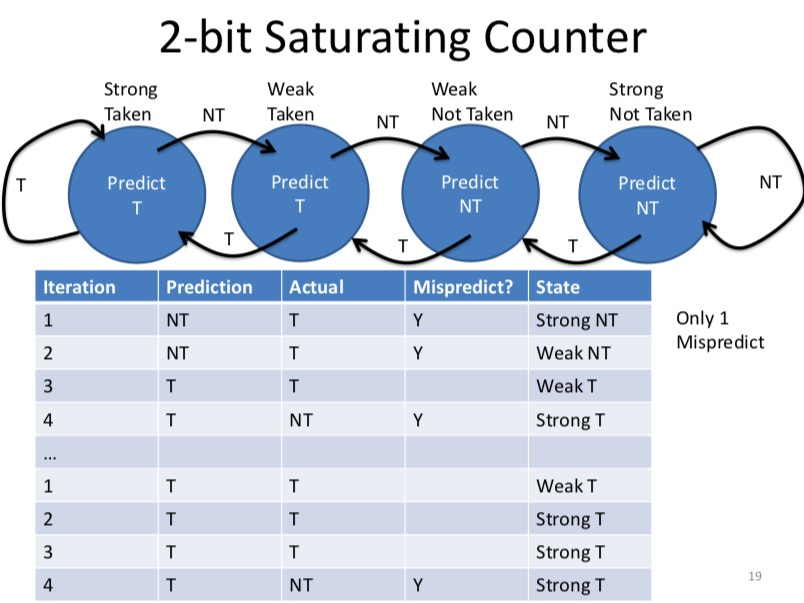
\includegraphics[height=100pt]{figure/2_bit_saturating.jpg}}
    \onslide<3->{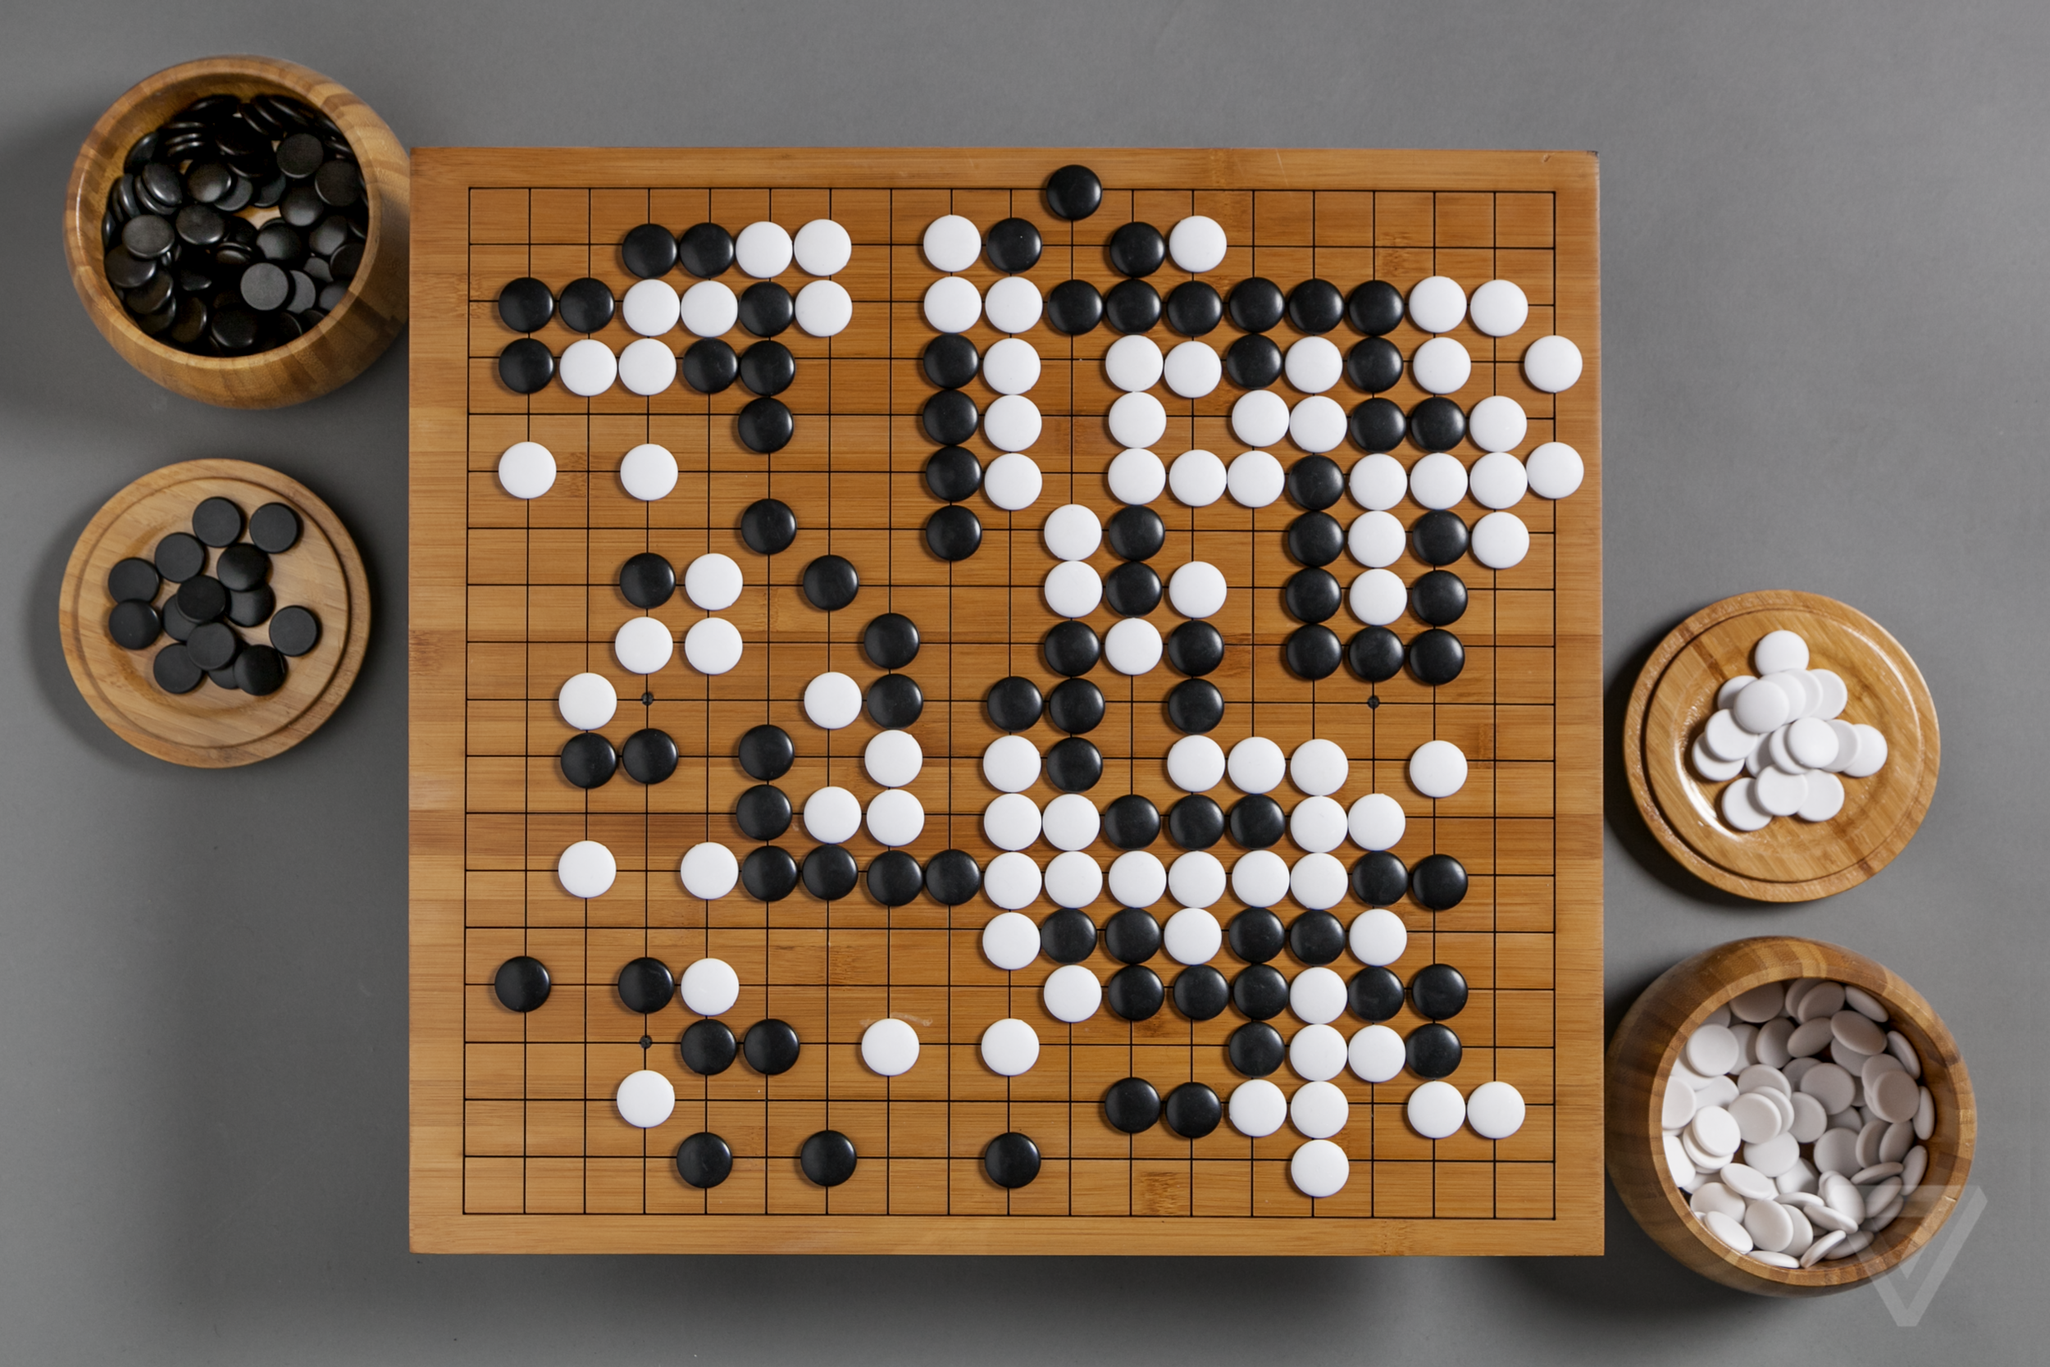
\includegraphics[height=100pt]{figure/go_pic.png}}
  \end{center} 
\end{frame}

\begin{frame}{How can AI promote our research of computer system?}
  And it turns out that...\footfullcite{zouzias2021branch}\footfullcite{silver2017mastering}
  \begin{center} 
    \onslide<2->{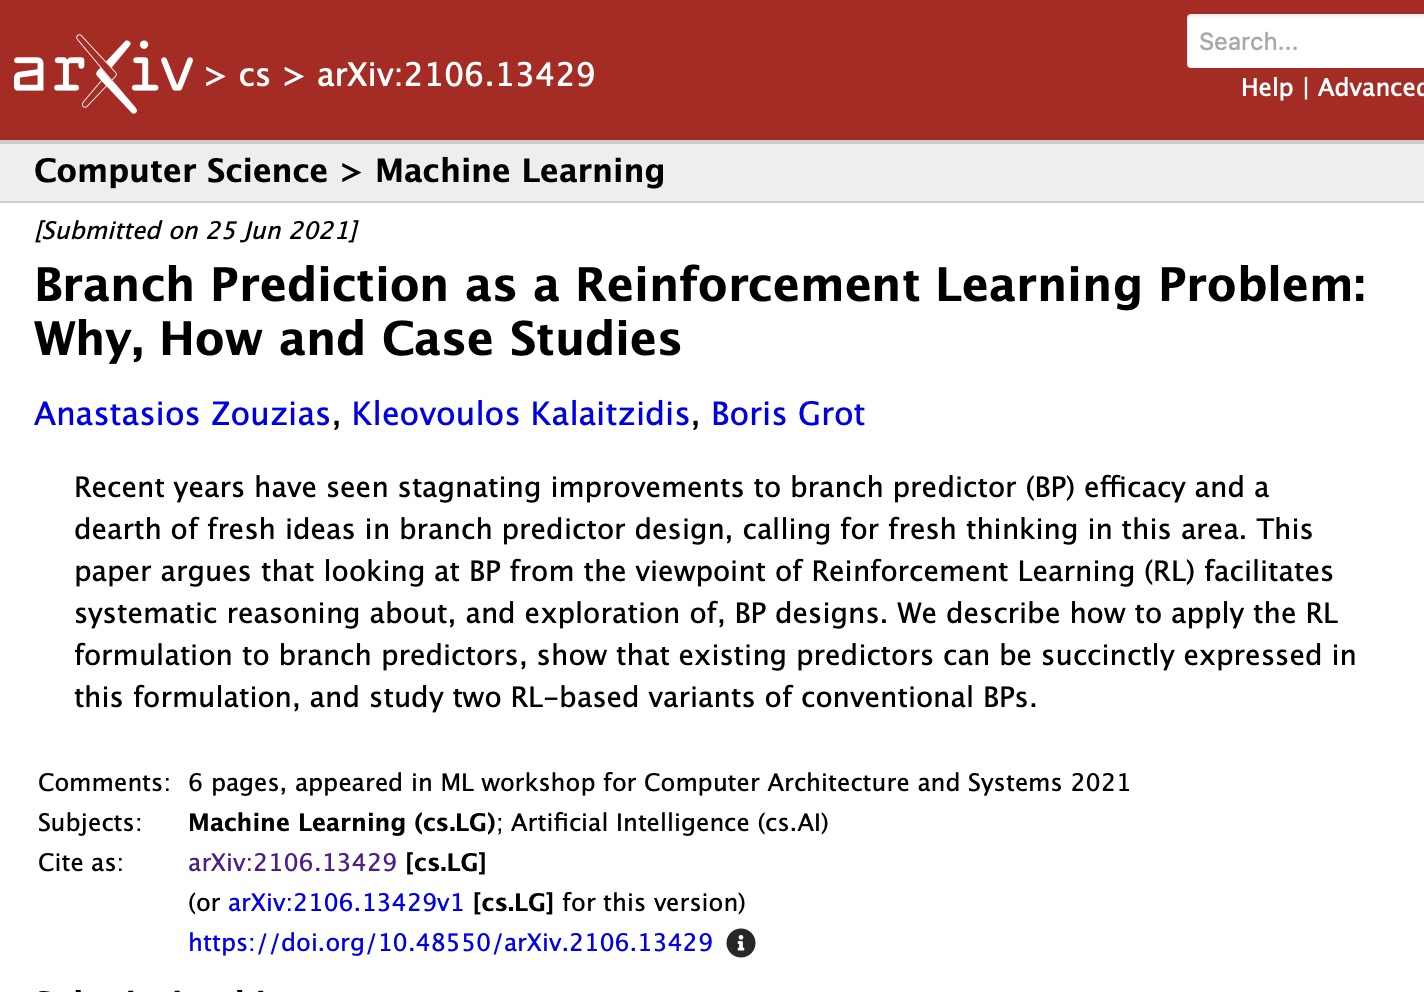
\includegraphics[height=100pt]{figure/reinforcement_prediction.png}}
    \onslide<3->{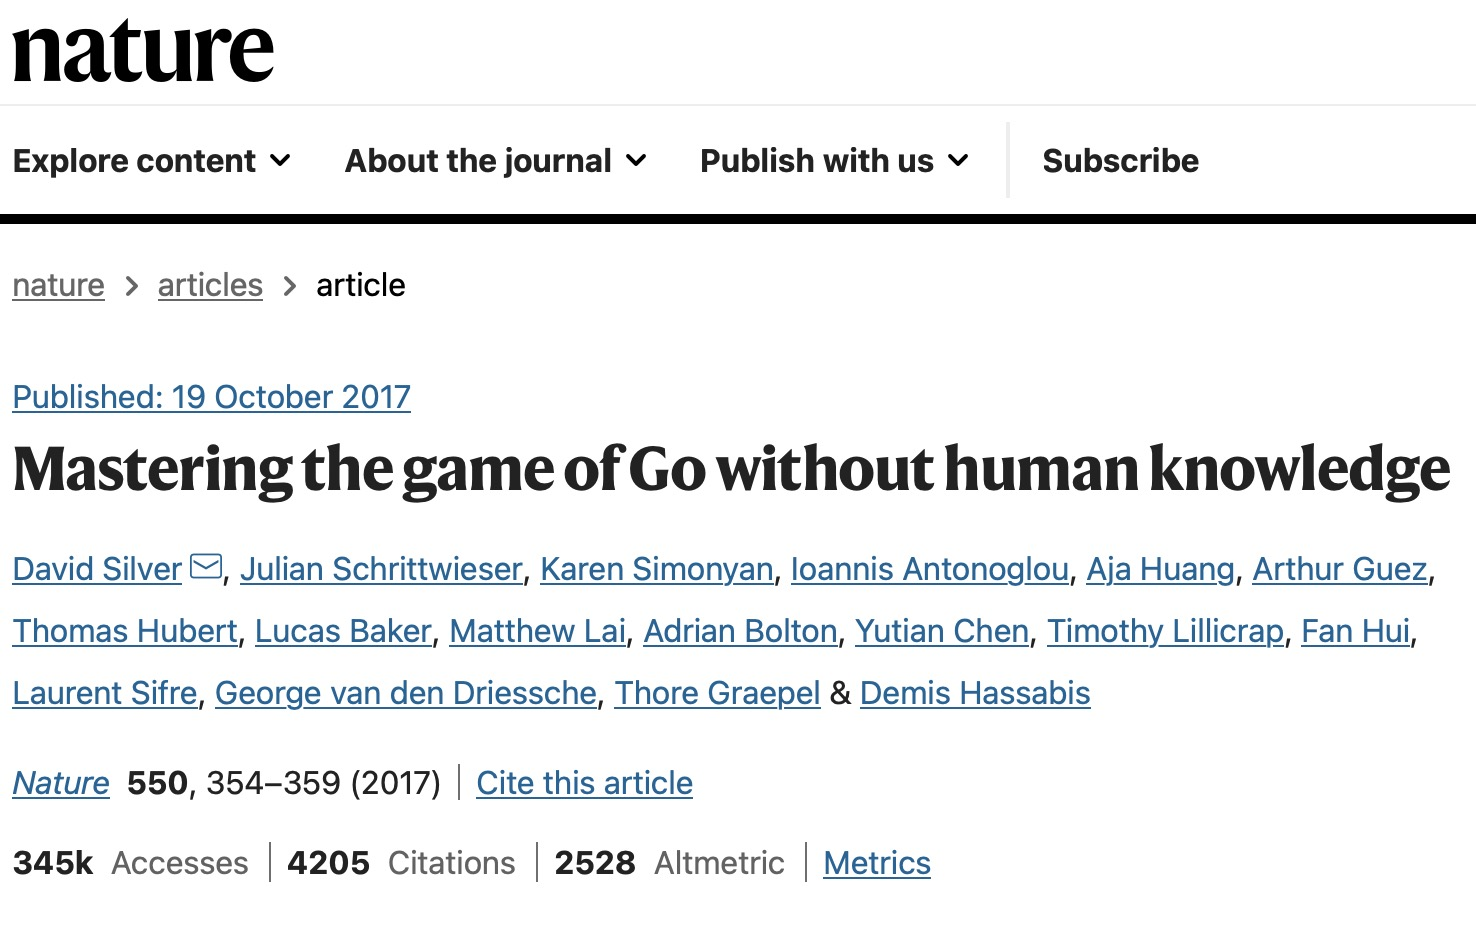
\includegraphics[height=100pt]{figure/master_go.png}}
  \end{center} 
\end{frame}

\begin{frame}{How can AI promote our research of computer system?}
  Their similarities:
  \begin{enumerate}
    \item<2-> Decision-making problems
    \item<3-> A finite state given as input
    \item<4-> A simple decision required as output
  \end{enumerate}

  \onslide<5->{The role that AI plays: looking for a fitting function $y=f(x)$, which calculates the correct/best $y$ with given $x$.}
\end{frame}

\begin{frame}{How does AI perform its job?}
  The perceptron is introduced at first:\footfullcite{jimenez2001dynamic}
  \begin{center} 
    \onslide<2->{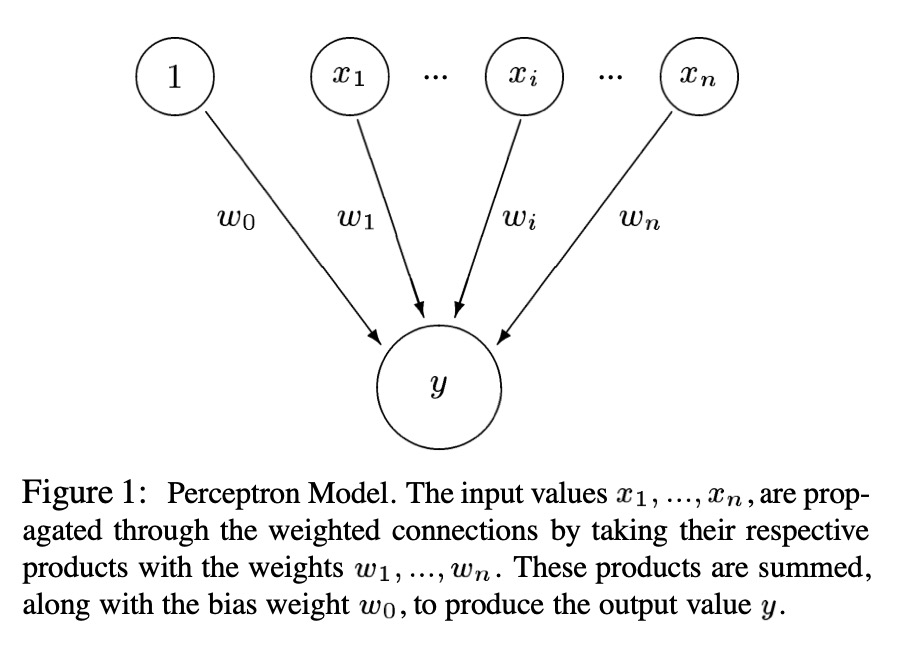
\includegraphics[height=120pt]{figure/perceptron.jpg}}
    \onslide<3->{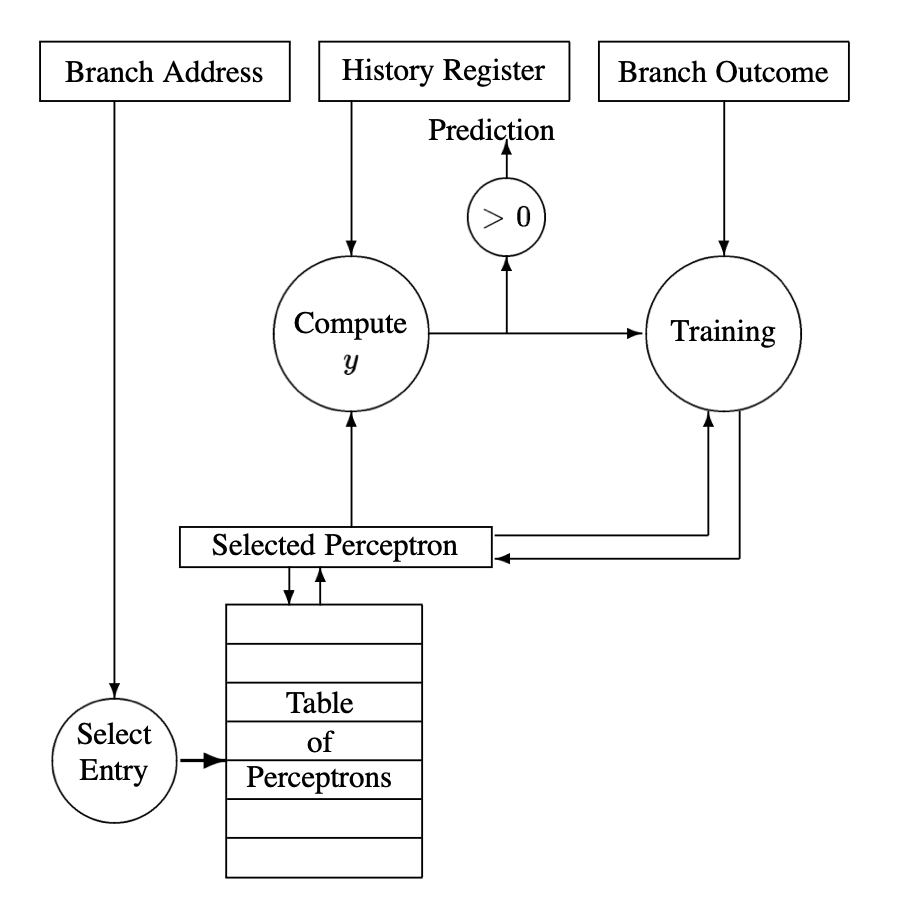
\includegraphics[height=120pt]{figure/bp_structure.png}}
  \end{center}
\end{frame}

\begin{frame}{Applications}
  AMD Zen microarchitecture, the start of "AMD YES".
  \begin{center}
    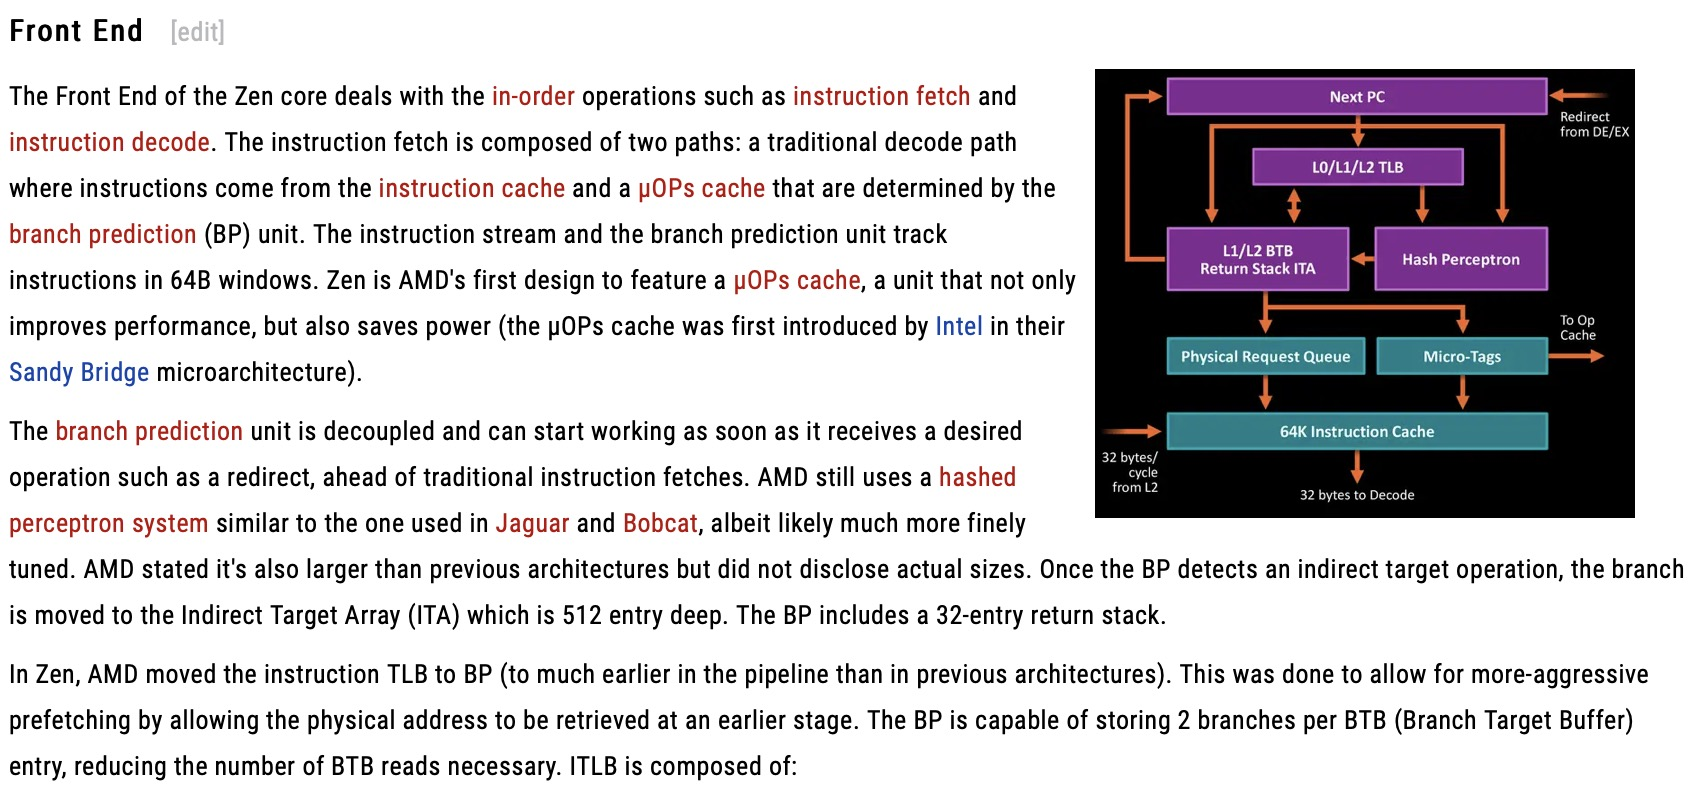
\includegraphics[height=150pt]{figure/amd_zen_bp.jpg}
  \end{center}
\end{frame}

\begin{frame}{Advanced version}
  Advanced neural network is also being introduced to many subfields of computer system\dots
\end{frame}

\begin{frame}{Reinforcement is what you need}
  Let's go over the basic concept of reinforcement learning.
  \begin{itemize}
    \item <2-> A virtual agent who makes decisions
    \item <3-> A state space $S=\{s_i\}$
    \item <4-> An action space $A=\{a_i\}$
    \item <5-> Rewards $r_{a_i|s_i}$
  \end{itemize}
  When agent receives a reward or a feedback, it updates its estimation or probability \begin{align*}
    \mathbb{E} (r_{a_i|s_i}), \mathbb{P} (r_{a_i|s_i}>0)
  \end{align*}
\end{frame}

\section{System for AI}

\begin{frame}{How can our works on computer system promote research of AI?}
  Key idea: build systems to adapt, simplify and accelerate machine learning.
\end{frame}

% \begin{frame}{}

% \begin{frame}
%     \kaishu
%     基本内容\par 
%     \begin{itemize}
%         \item 1. 引言
%         \item 2. 绪论
%         \item 3. 定理的证明
%     \end{itemize}
% \end{frame}

% \section{彩色强调背景}
% \begin{frame}
%     常见的微分方程
%     % \begin{tcolorbox}[colback=blue!5!white,colframe=blue!75!black,title=ODES Ordinary Form]
%         \begin{align}
%             \mbox{标准形式}\frac{dy}{dx} + &p(x)=q(x)\nonumber\\
%             &\mbox{通解}y=e^{-\int_{}^{}{p(x)dx}}\cdot\int_{}^{}{[e^{\int_{}^{}{p(x) dx}} \cdot q(x)+C] dx}
%       \end{align}
%     % \end{tcolorbox}
%     % \textcolor{blue!70}{
%         \kaishu
%         \fontsize{7pt}{2pt}
%     明显的自己的tcolorbox没有beamer中自带的therom环境的样式协调
%     % }
% \end{frame}

% \section{分栏}
% \begin{frame}{A sample slide In Multi columns}
% 在 Beamer 中的 columns 环境提供了一个简便的方法将幻灯片分成数栏。
% 这在幻灯片中放置图片或创建多栏(multi-column)
% 常规列表(itemized lists)时特别有用。

%     \begin{theorem}[The Poincar\'e inequality]
%         Suppose $\Omega\in\mathbf{R}^n$ is a bounded domain with smooth
%         boundary.  Then there exists a $\lambda>0$, depending only on
%         $\Omega$, such that for any function $f$ in the Sobolev space
%         $H^1_0(\Omega)$ we have:
        
%         \[
%         \int_\Omega |\nabla u|^2 \,dx \ge 
%         \lambda \int_\Omega |u|^2 \,dx .
%         \]
%     \end{theorem}
%     Here is what \emph{itemized} and \emph{enumerated} lists look like:
%     \begin{columns}
%       \begin{column}{0.45\textwidth}
%       \begin{itemize}
%         \item itemized item 1
%         \item itemized item 2
%         \item itemized item 3
%       \end{itemize}
%       \end{column}
    
%       \begin{column}{0.45\textwidth}
%       \begin{enumerate}
%         \item enumerated item 1
%         \item enumerated item 2
%         \item enumerated item 3
%       \end{enumerate}
%       \end{column}
%     \end{columns}
% \end{frame}

% % \begin{frame}{II}
% %   观察上述的示例幻灯片,两栏的垂直中心点(vertical mid-points)是水平对齐的。
% % 这时,我们简称栏是中心对齐的(center-aligned)。

% % columns 环境的 [t] 选项,即 \textbackslash begin{columns}[t],
% % 使栏顶部对齐(top-aligned)。选项 [b] 使栏底部对齐(bottom-alignment),
% % 选项 [c] 使栏中心对齐(center-alignment)(这是默认选项) 。
% % 下面的例子栏是顶部对齐的:
% % \end{frame}

% \begin{frame}{Splitting a slide into columns}

%   The line you are reading goes all the way across the slide.
%   From the left margin to the right margin.  Now we are going
%   the split the slide into two columns.
%   \bigskip
  
%   \begin{columns}
%     \begin{column}{0.5\textwidth}
%       Here is the first column.  We put an itemized list in it.
%       \begin{itemize}
%         \item This is an item
%         \item This is another item
%         \item Yet another item
%       \end{itemize}
%     \end{column}
  
%     % \begin{column}{0.3\textwidth}
%     %   Here is the second column.  We will put a picture in it.
%     %   \centerline{\includegraphics[width=0.7\textwidth]{../Pic/cover.jpg}}
%     % \end{column}
%   \end{columns}
%   \bigskip
  
%   The line you are reading goes all the way across the slide.
%   From the left margin to the right margin.
%   \end{frame}

% \begin{frame}[t]{Top alignment} 
%   This is the contents of the slide. 
% \end{frame} 
  
% \begin{frame}[c]{Center alignment (default)} % [c] 是默认的
%   This is the contents of the slide. 
% \end{frame} 

% \begin{frame}[b]{Bottom alignment} 
%   This is the contents of the slide. 
% \end{frame} 

% \begin{frame}[t]{字号设置}
%   Beamer 的默认字体尺寸是 11 点(points)。 
%   在 \textbackslash documentclass 这一行,可以设定默认字体尺寸为 
%   8、9、10、11、 12、14、17、20点。
%   例如,要设定默认的字体尺寸为 14 点,请这样做:
%   \rule{0.6\linewidth}{1pt}

%   \bigskip
%   \textbackslash \texttt{documentclass[14pt]\{beamer\}}
%   % \documentclass[14pt]{beamer} 
% \end{frame}


% \section{图片}
% % \begin{frame}{插入图片}
% %   下边插入了一个pdf和一个jpg的图片文件
% %   \begin{center} 
% %     \includegraphics[width=0.3\textwidth]{../Pic/cover.jpg} 
% %     \includegraphics[width=0.3\textwidth]{../Pic/上下极限散点图.pdf} 
% %   \end{center}  
% % \end{frame}

% % \begin{frame}{TiKZ in Beamer}
% %   \begin{figure}[!htb]
% %     \begin{minipage}[]{0.4\linewidth}
% %         如右图所示:
% %         \begin{itemize}
% %             \item 1. $M$就是阴影区域 $f(x, y)$的最大值
% %             \item 2. $y=\varphi(x)$的唯一性在 $x\in [x_0-h, x_0+h]$上能够保证
% %         \end{itemize}
% %     \end{minipage}
% %     \begin{minipage}[]{0.4\linewidth}
% %         \center
% %         \begin{tikzpicture}{scale=0.07}
% %             \draw[-stealth] (-1, 0)--(5, 0)node[below=.5em, left] {$x$};
% %             \draw[-stealth] (0, -1)--(0, 5)node[right=.5em, below] {$y$};
% %             \draw[fill = black!20] (1, 1)--(4, 1)--(4, 3)--(1, 3)--cycle;
% %             \draw[dashed] (2.5, 0)node[below] {$x_0$}--(2.5, 2)node[right=.5em, above=.25em] {$(x_0, y_0)$}--(0, 2)node[left] {$y_0$};
% %             \draw[decorate, decoration={calligraphic brace, amplitude=2mm}] (1, 3)--(4, 3)node[midway, above=.5em] {$2a$};
% %             \draw[decorate, decoration={calligraphic brace, mirror, amplitude=2mm}] (4, 1)--(4, 3)node[midway, right=.5em] {$2b$};
% %             \node[left=.5em, below] at (0, 0) {$O$};
% %             \draw[fill=black!60]  (2.5, 2) circle (2pt);
% %             \draw[dashed] (2.2, 0)--(2.2, 2);
% %             \draw[dashed] (2.8, 0)--(2.8, 2)--(2.5, 2);
% %             \draw[decorate, decoration={calligraphic brace}] (2.2, 0)--(2.8, 0)node[midway, above=.5em] {$2h$};
% %         \end{tikzpicture}
% %     \end{minipage}
% % \end{figure}
% % \end{frame}

% \section{叠层显示:幻灯片逐渐显示}
% \begin{frame}{Outline of the talk} 
%   \begin{itemize} 
%     \item Introduction 
%     \pause 
%     \item Statement of the main theorem 
%     \pause 
%     \item Technical lemmata 
%     \pause 
%     \item Proof of the main theorem 
%     \pause 
%     \item Conclusions 
%   \end{itemize} 
% \end{frame} 
  
% % \section{更加复杂的放映规则}
% \begin{frame}{Fermat's Last Theorem} 
 
%   In this talk I will give a very elementary proof of the 
%   theorem.  I am surprised that no one else has thought of 
%   this before. 
%   \medskip 
   
%   \pause 
   
%   Fermat's Last Theorem says that the equation 
%   \[ 
%     x^2 + y^2 = z^2 
%   \] 
%   has no solution in the set of natural numbers. 
%   \medskip 
   
%   \pause 
   
%   This is not true.  After a lengthy calculation on the 
%   department's Linux machines, I have verified that within 
%   the numerical accuracy of the Pentium-4 processor, we have: 
%   \[ 
%     5000^2 + 12000^2 = 13000^2 
%   \] 
   
%   \end{frame} 
% %% 最多6个目录
% \section{跳转}
% \begin{frame}[label=intro]{Introduction}

%   This slide is labeled ``intro''.
  
%   \end{frame}
  
%   %--- 帧 --------------------------------------------------%
%   \begin{frame}{Some other slide}
  
%   If you click \hyperlink{intro}{here}, you will jump to the slide
%   labeled ``intro''.
  
%   \bigskip
  
%   Clicking \hyperlink{intro}{\beamerbutton{here}} will also
%   take you to the ``intro'' slide.

%   \medskip

%   \textbf{注:使用Alt + $\leftarrow$跳转回来}

%   \bigskip

%   \textbf{注:在pdf文件关闭的情况下写入,此时pdf文件被锁死了,无法写入}
%   \end{frame}
  

% \begin{frame}{使用脚注}
%   Fnote 环境带有两个参数,它们指定了脚步注的位置即相对于
%   幻灯片的左上角。 一张 Beamer 幻灯片的大小是 128mm $\times$ 96mm。
%   这有利于你设定这些参数。


% %  \begin{Fnote}{4mm}{80mm}
% %       V. Jikov, S. Kozlov and O. Olenik, Homogenization
% %       of differential operators and integral
% %       functionals, Springer, 1994.
% %   \end{Fnote} 
% \end{frame}

% % \begin{frame}{数学公式字体}
% %   打字机字体:\\
% %   \begin{center}
% %     \texttt{Hello world from \LaTeX}
% %   \end{center}
% %   数学公式粗体:
% %   \[
% %     a+b\times c \ne \boldsymbol{a+b \times c}
% %   \]
% %   数学公式伪粗体:
% %   \[
% %     \int k =  \pmb{\int k}  
% %   \]
% %   高质量粗体:
% %   \[
% %     \sum \int (k\oplus j) \,{d}x \ne
% %     \bm{\sum \int (k\oplus j) \,{d}x}
% %   \]
% % \end{frame}

% \begin{frame}[shrink=50]{Frame 的缩放} 
%   一大段的文字:\par 
%   这将按比例缩小幻灯片的内容至少 50\% ,如果需要,还能缩小更多,
%   直至内容完全能被幻灯片所容纳。

% 为达到最佳效果,你指定的缩小因子应尽可能接近所需的数值。
% 如果你指定的缩小因子的值不合适,Beamer 将发出警告。
% 调整缩小因子直至警告消失。然而,幻灯片的水平间隙
% (horizontal spacing)将不是最佳的。

% 你不应滥用这个缩小功能——少量的缩小不会引人注意,到处都使用了
% 缩小就会让人看着不愉快。

% \vspace*{5em}
% \begin{flushleft}
%   \Huge
  
%   字体的前景与背景高亮\par
  
%   \vspace*{2em}
%   \Large
%   \colorbox{red}{This text is highlighted in red}

%   \textcolor{blue}{This text is in blue}
% \end{flushleft}

% \end{frame} 
  
  

\end{document}